%-------------------------------------------------------------
%---------------------- Apêndices ----------------------------
%-------------------------------------------------------------
%Note que os Apêndices são dedicados aos textos ou \textbf{documentação elaborados pelo próprio autor} que complemente  a  argumentação  textual  (códigos,  reportagens,  relatórios  etc.).

\titlespacing*{\chapter}{0pt}{-10pt}{-2cm} 
\captionsetup[figure]{list=no} % Remove as figuras da lista
%\captionsetup[table]{list=no} % Remove as tabelas da lista

%\partapendices  % Indica o início dos Apendices

\chapter*{Apêndice A - Propriedades Mecânicas do AISI/SAE 4340}
\label{apendiceA}

\begin{figure}[h]
   \centering
    \caption{Propriedades do material no ANSYS Mechanical.}
    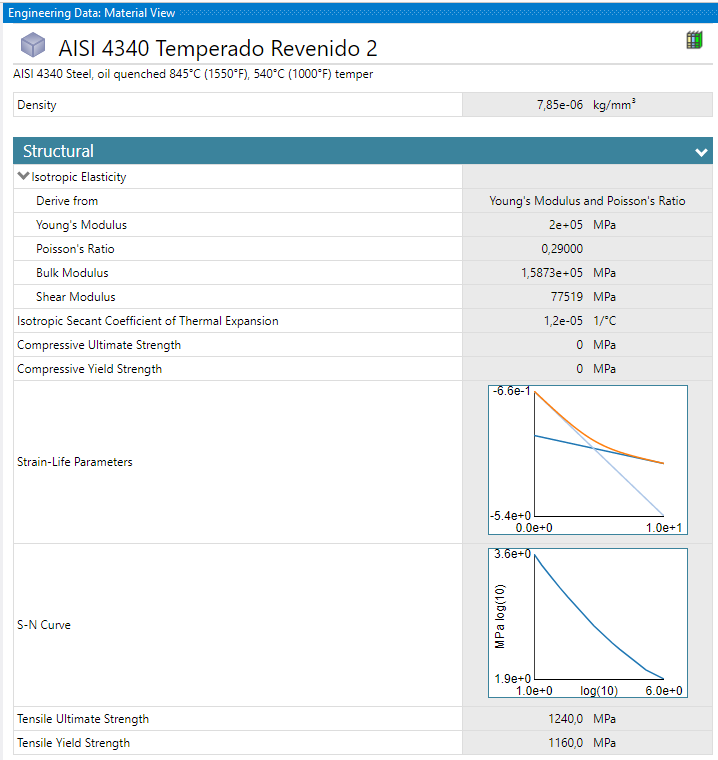
\includegraphics[width=1.0\linewidth, trim = 0 0 0 0, clip]{Figuras/4340Ansys2.png}\\
    \hspace{1.5cm}\raggedright \fontsize{10}{12}\selectfont{Fonte: Elaborado pelo autor, 2025.}
    \label{4340Ansys}
\end{figure}



